\documentclass[12pt, titlepage]{article}

\usepackage{fullpage}
\usepackage[round]{natbib}
\usepackage{multirow}
\usepackage{booktabs}
\usepackage{tabularx}
\usepackage{graphicx}
\graphicspath{ {./images/} }
\usepackage{float}
\usepackage{hyperref}
\hypersetup{
    colorlinks,
    citecolor=blue,
    filecolor=black,
    linkcolor=red,
    urlcolor=blue
}

%% Comments

\usepackage{color}

\newif\ifcomments\commentstrue %displays comments
%\newif\ifcomments\commentsfalse %so that comments do not display

\ifcomments
\newcommand{\authornote}[3]{\textcolor{#1}{[#3 ---#2]}}
\newcommand{\todo}[1]{\textcolor{red}{[TODO: #1]}}
\else
\newcommand{\authornote}[3]{}
\newcommand{\todo}[1]{}
\fi

\newcommand{\wss}[1]{\authornote{blue}{SS}{#1}} 
\newcommand{\plt}[1]{\authornote{magenta}{TPLT}{#1}} %For explanation of the template
\newcommand{\an}[1]{\authornote{cyan}{Author}{#1}}

%% Common Parts

\newcommand{\progname}{ProgName} % PUT YOUR PROGRAM NAME HERE
\newcommand{\authname}{Team \#, Team Name
\\ Student 1 name
\\ Student 2 name
\\ Student 3 name
\\ Student 4 name} % AUTHOR NAMES                  

\usepackage{hyperref}
    \hypersetup{colorlinks=true, linkcolor=blue, citecolor=blue, filecolor=blue,
                urlcolor=blue, unicode=false}
    \urlstyle{same}
                                


\newcounter{acnum}
\newcommand{\actheacnum}{AC\theacnum}
\newcommand{\acref}[1]{AC\ref{#1}}

\newcounter{ucnum}
\newcommand{\uctheucnum}{UC\theucnum}
\newcommand{\uref}[1]{UC\ref{#1}}

\newcounter{mnum}
\newcommand{\mthemnum}{M\themnum}
\newcommand{\mref}[1]{M\ref{#1}}

\begin{document}

\title{System Design for \progname{}} 
\author{\authname}
\date{\today}

\maketitle

\pagenumbering{roman}

\section{Revision History}

\begin{tabularx}{\textwidth}{p{3cm}p{2cm}X}
\toprule {\bf Date} & {\bf Version} & {\bf Notes}\\
\midrule
Date 1 & 1.0 & Notes\\
Date 2 & 1.1 & Notes\\
\bottomrule
\end{tabularx}

\newpage

\section{Reference Material}

This section records information for easy reference.

\subsection{Abbreviations and Acronyms}

\renewcommand{\arraystretch}{1.2}
\begin{tabular}{l l} 
  \toprule		
  \textbf{symbol} & \textbf{description}\\
  \midrule 
  \progname & Explanation of program name\\
  \wss{...} & \wss{...}\\
  \bottomrule
\end{tabular}\\

\newpage

\tableofcontents

\newpage

\listoftables

\listoffigures

\newpage

\pagenumbering{arabic}

\section{Introduction}

\wss{Include references to your other documentation}

\section{Purpose}

\wss{Purpose of your design documentation}

\wss{Point to your other design documents}

\section{Scope}

\wss{Include a figure that show the System Context (showing the boundary between
your system and the environment around it.)}

\section{Project Overview}

\subsection{Normal Behaviour}

\subsection{Undesired Event Handling}

\wss{How you will approach undesired events}

\subsection{Component Diagram}

\subsection{Connection Between Requirements and Design} \label{SecConnection}

\wss{The intention of this section is to document decisions that are made
  ``between'' the requirements and the design.  To satisfy some requirements,
  design decisions need to be made.  Rather than make these decisions implicit,
  they are explicitly recorded here.  For instance, if a program has security
  requirements, a specific design decision may be made to satisfy those
  requirements with a password.}

\section{System Variables}

\wss{Include this section for Mechatronics projects}

\subsection{Monitored Variables}

\subsection{Controlled Variables}

\subsection{Constants Variables}

\section{User Interfaces}

\wss{Design of user interface for software and hardware.  Attach an appendix if
needed. Drawings, Sketches, Figma}

The User Interface will consist of a set of buttons to allow the operator to safely 
interact with the machine. It will also consist of audible and visual signals to alert
the operator of any action required (e.g. tray/pot restock, verification error, etc.).
See Appendix A for interface layout concept.

\section{Design of Hardware}

\wss{Most relevant for mechatronics projects}
\wss{Show what will be acquired}
\wss{Show what will be built, with detail on fabrication and materials}
\wss{Include appendices as appropriate, possibly with sketches, drawings, CAD, etc}
\subsection{Conveyor}

The conveyor subsystem will be comprised of:
\begin{itemize}
  \item 1 conveyor (including belt, motor, gear box and framing)
  \item 1 Arduino Uno microcontroller
  
\end{itemize}
The conveyor has been acquired from Sheridan Nurseries and will not require fabrication.


\subsection{Pot Dropper}

The pot dropper subsystem will be comprised of:
\begin{itemize}
  \item 4 stepper motors
  \item 4 stepper motor drivers
  \item 1 Arduino Uno microcontroller
  \item 4 pot dropper screws
  \item 1 ultrasonic range finder
\end{itemize}
The pot dropper will be fabricated with steel x-beam framing to support the mechanism.
See Appendix B.1 for a CAD diagram of the pot dropper screw.

\subsection{Tray Dropper}

The tray dropper subsystem will be comprised of:
\begin{itemize}
  \item 2 stepper motors
  \item 2 belts
  \item 4 belt bearings
  \item 1 steel x-beam frame
  \item 1 tray dropper end-effector
\end{itemize}
The tray dropper will be fabricated with x-beam framing to support the mechanism. The 
stepper motors and belt bearings will be attached to the framing, and the belts will 
be secured to the bearings. See Appendix B.2 for a CAD diagram of the tray dropper 
end-effector.

\subsection{Tray Elevator}

The tray elevator will be comprised of:
\begin{itemize}
  \item 4 L-shaped wood frame supports
  \item 4 long wood frame supports
  \item 4 short wood frame supports
  \item 1 wood raising platform
  \item 1 ultrasonic range finder
  \item 2 spur gears
  \item 2 racks
  \item 2 stepper motors
\end{itemize}
The wooden frame will be fabricated with screws and wood glue. The stepper motors 
will be attached to either side of the wood platform responsible for hodling the 
stack of trays. The spur gears will be attached to the stepper motors. The racks 
will be attached in the centre of the long wood supports on either side of the frame, 
and will mesh with the spur gears. This will enable the stepper motors to control the 
lifting and lowering of the tray elevator based on its current capacity (see Appendix B.3
for CAD diagram).

\subsection{Verification}

The verification subsystem will be comprised of:
\begin{itemize}
  \item 1 ultrasonic range finder
\end{itemize}

\section{Design of Electrical Components}

\wss{Most relevant for mechatronics projects}
\wss{Show what will be acquired}
\wss{Show what will be built, with detail on fabrication and materials}
\wss{Include appendices as appropriate, possibly with sketches, drawings,
circuit diagrams, etc}

\section{Design of Communication Protocols}

\wss{If appropriate}

\section{Timeline}

\wss{Schedule of tasks and who is responsible}

% \bibliographystyle {plainnat}
% \bibliography{../../../refs/References}

\newpage{}

\appendix

\section{Interface}

% \wss{Include additional information related to the appearance of, and
% interaction with, the user interface}


\includegraphics{interface1.png}
\newline
An example of a status message alerting the machine operator that the pot 
dispenser requires refill. This would be accompanied by an audible alert.

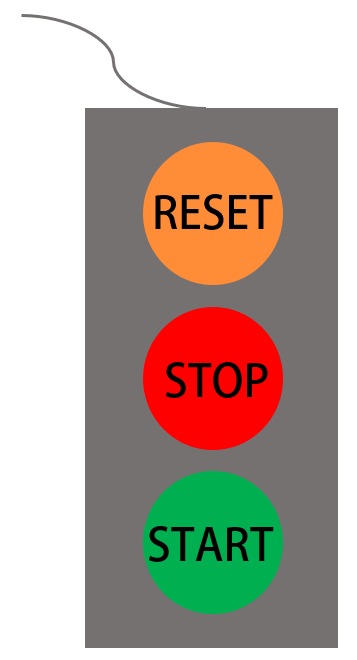
\includegraphics{interface2.png}
\newline
Concept of the button interface used by the operator to control the machine. 
Handheld as to mitigate any safety concerns with a machine-mounted apparatus.

\section{Mechanical Hardware}

\subsection{Pot Dropper}

\subsection{Tray Dropper}

\subsection{Tray Elevator}

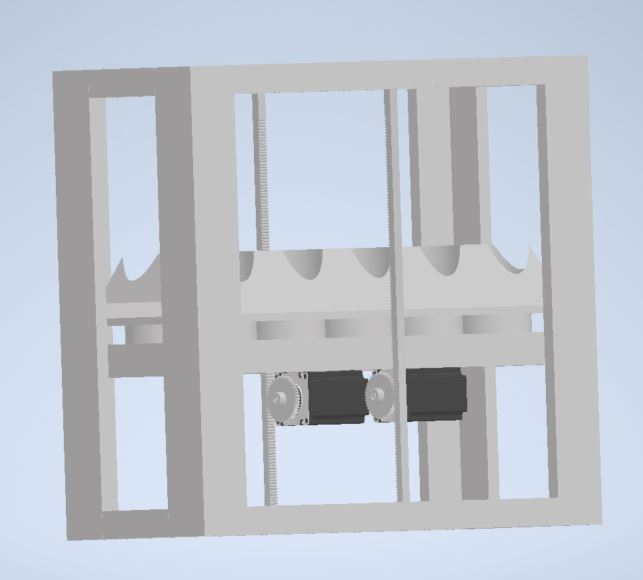
\includegraphics{Tray_Elevator.jpg}
\newpage
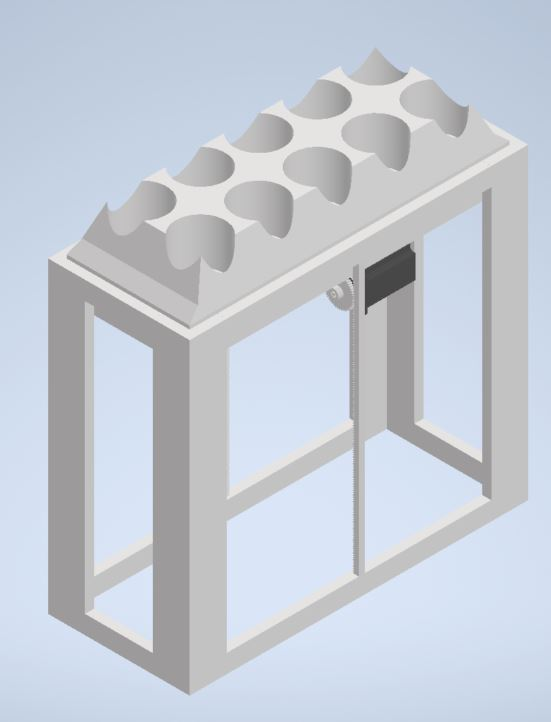
\includegraphics{Tray_Elevator2.jpg}

\section{Electrical Components}

\section{Communication Protocols}

\section{Reflection}

The information in this section will be used to evaluate the team members on the
graduate attribute of Problem Analysis and Design.  Please answer the following questions:

\begin{enumerate}
  \item What are the limitations of your solution?  Put another way, given
  unlimited resources, what could you do to make the project better? (LO\_ProbSolutions)
  \item Give a brief overview of other design solutions you considered.  What
  are the benefits and tradeoffs of those other designs compared with the chosen
  design?  From all the potential options, why did you select documented design?
  (LO\_Explores)
\end{enumerate}

\end{document}